%%%%%%%%%%%%%%%%%%%%%%%%%%%%%%%%%%%%%%%%%%%%%%%%%%%%%%
% A Beamer template for Ritsumeikan University       %
% Author: Ming-Hao Xu (Xu Minghao)                   %
% Date:   April 2022.                                %
% LPPL Licensed.                                     %
%%%%%%%%%%%%%%%%%%%%%%%%%%%%%%%%%%%%%%%%%%%%%%%%%%%%%%

\documentclass{beamer}
\usepackage{hyperref}

\usepackage[UTF8]{ctex}
\usepackage[T1]{fontenc}

% other packages
\usepackage{latexsym,amsmath,xcolor,multicol,booktabs,calligra}
\usepackage{graphicx,pstricks,listings,stackengine}
\usefonttheme[onlymath]{serif}

% dummy text; remove it when working on this template
\usepackage{lipsum}

\author{Ebola}
\title{最优化选讲:凸优化与模拟退火}
\institute{
    Institute of Mathematics, \\
    Zhejiang University.
}
\date{Jan, 2024}
\usepackage{Ritsumeikan}

% defs
\def\cmd#1{\texttt{\color{red}\footnotesize $\backslash$#1}}
\def\env#1{\texttt{\color{blue}\footnotesize #1}}
\definecolor{deepblue}{rgb}{0,0,0.5}
\definecolor{deepred}{rgb}{0.6,0,0}
\definecolor{deepgreen}{rgb}{0,0.5,0}
\definecolor{halfgray}{gray}{0.55}

\lstset{
    basicstyle=\ttfamily\tiny,
    keywordstyle=\bfseries\color{deepblue},
    emphstyle=\ttfamily\color{deepred},    % Custom highlighting style
    stringstyle=\color{deepgreen},
    numbers=left,
    numberstyle=\small\color{halfgray},
    rulesepcolor=\color{red!20!green!20!blue!20},
    frame=shadowbox,
}


\begin{document}

\begin{frame}
    \titlepage
\end{frame}

\begin{frame}
    \tableofcontents[sectionstyle=show,subsectionstyle=show/shaded/hide,subsubsectionstyle=show/shaded/hide]
\end{frame}

\section{凸优化}

\begin{frame}{问题形式}
    \small
    给定一个函数 $f(x)$,求 $f(x)$ 在 $[l,r]$ 中的最小值。
\end{frame}

\begin{frame}{凸集}
    \small
    在一个平面上,如果一个区域中任意两点之间的连线都落在这个区域内,我们就说这个区域是“凸集”。
    \begin{figure}[H]
        \centering
        
\includegraphics[width=0.9\textwidth]{pic/convexRegion.png}
    \end{figure}
\end{frame}

\begin{frame}{凸函数}
    \small
    函数图像 $y=f(x)$ 将平面直角坐标系分割成上下两个部分,如果上半部分是凸集,那么我们就说 $f(x)$ 是凸函数。 
    \begin{itemize}
        \item 抛物线 $f(x)=x^2$ 是凸函数;
        \item 对勾函数 $f(x)=x+\frac{1}{x}\;(x>0)$ 是凸函数;
        \item 负对数 $f(x)=-\ln x\; (x>0)$ 是凸函数;
        \item 三角函数 $f(x)=\sin x$ 不是凸函数。
    \end{itemize}

    \begin{figure}[H]
        \centering
        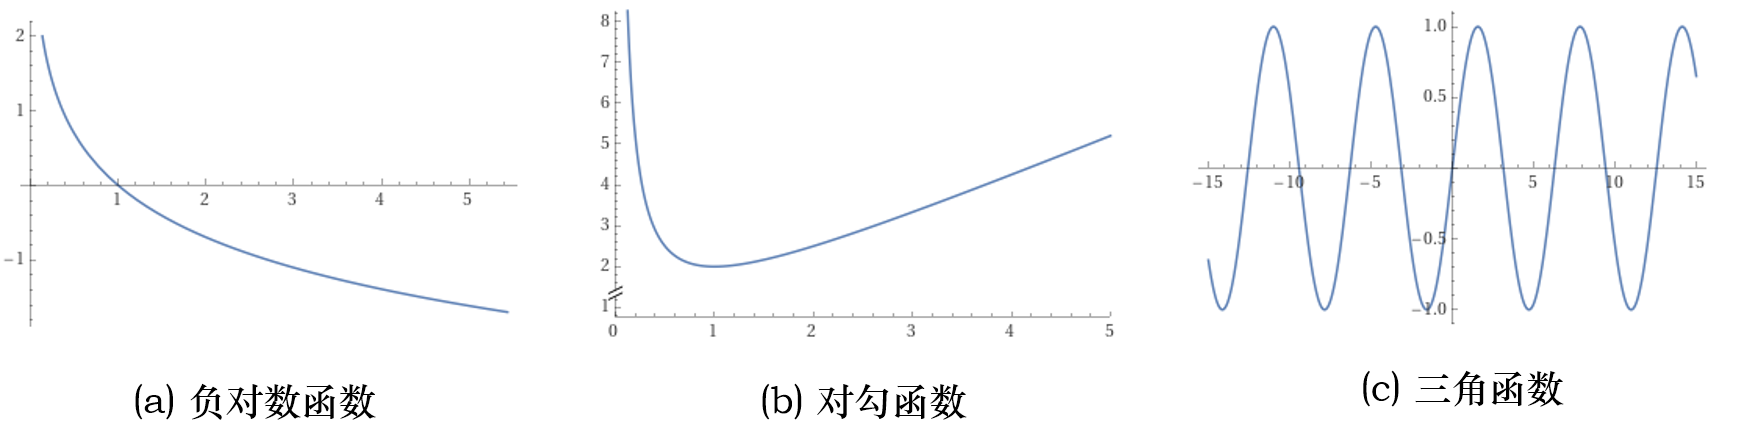
\includegraphics[width=0.9\textwidth]{pic/convexFunction.png}
    \end{figure}

    \pause
    如果 $[l,r]$ 在凸函数 $f(x)$ 的定义域内,那么 $f(x)$ 在 $[l,r]$ 中存在唯一的最小值点。
\end{frame}

\begin{frame}[fragile]{求凸函数的最小值}
    \small
    给定一个凸函数 $f(x)$,求 $f(x)$ 在 $[l,r]$ 中的最小值。
    \vspace{2em}

    \pause
    三分法。
    \begin{lstlisting}[language=c++]
        double search(double l, double r)
        {
            double mid1 = l + (r-l) / 3;
            double mid2 = r - (r-l) / 3;
            while(mid2-mid1 > 1e-9)
            {
                if(f(mid1) > f(mid2)) l = mid1;
                else r = mid2;
                mid1 = l + (r-l) / 3;
                mid2 = r - (r-l) / 3;
            }
            return l;
        }
    \end{lstlisting}
    \vspace{2em}

    \pause
    习题:【P1883】函数
\end{frame}

\begin{frame}[fragile]{求凸函数的最小值}
    \footnotesize
    一种卡常到极致的方法:0.618法。令:
    \begin{equation*}
        c=\frac{\sqrt{5}-1}{2}(\approx 0.618),
    \end{equation*}
    可以验证,$1-c^2=c$. 在区间 $[l,r]$ 中,我们取
    \begin{equation*}
        mid_1=r-c(r-l),\quad mid_2=l+c(r-l).
    \end{equation*}
    如果 $f(mid_1)>f(mid_2)$,就令 $l=mid_1$;否则 $r=mid_2$。

    \pause
    现在假设 $l=mid_1$ (另一种情况是类似的),那么下一步,我们有:
    \begin{equation*}
        mid'_1=r-c(r-mid_1),\quad mid'_2=mid_1+c(r-mid_1).
    \end{equation*}
    \pause 可以发现:
    \begin{align*}
        mid'_1&=r-c(r-mid_1)=r-c(r-(r-c(r-l)))=r-c^2(r-l)\\
        &=r-(1-c)(r-l)=l+c(r-l)=mid_2.
    \end{align*}
    所以不需要重复计算 $f(mid_1')$,只需要计算 $f(mid'_2)$ 即可。

    \pause
    \begin{itemize}
        \item 三分法每次将区间缩小到 $\frac{2}{3}$ 倍,每次循环需要算两个点的函数值;
        \item 0.618法每次将区间缩小到 $0.618$ 倍,每次循环只要算一个点的函数值。
    \end{itemize}
    当函数值的计算复杂度为 $O(n)$ 时,0.618法能带来巨大优势。
\end{frame}


\begin{frame}[fragile]{求凸函数的最小值}
    \small
    0.618 法代码
    \begin{lstlisting}[language=c++]
        double search(double l, double r){
            const double c = (sqrt(5)-1)/2;
            double f1 = f(r - c * (r-l));
            double f2 = f(l + c * (r-l));
            while(r-l > 2e-8){
                if(f1 > f2){
                    l = r - c * (r-l);
                    f1 = f2;
                    f2 = f(l + c * (r-l));
                } else {
                    r = l + c * (r-l);
                    f2 = f1;
                    f1 = f(r - c * (r-l));
                }
            }
            return (l+r)/2;
        }
    \end{lstlisting}
\end{frame}


\begin{frame}{高维凸优化}
    \small
    以二维为例,给定一个函数 $f(x,y)$,定义域是 $x,y$ 为任意实数,求它的最小值。

    \vspace{1em}
    \pause
    选择一个方向 $(p,q)$,令 $g(t)=f(x+tp, y+tq)$,然后用三分(或0.618)法求 $g(t)$
    的最小值。然后换一个方向重复上述过程,直到充分接近最小值点为止。
    \pause
    \begin{itemize}
        \item 最速下降法:每次选择负梯度方向,即 $p=-\frac{\partial f}{\partial x}(x,y), q=-\frac{\partial f}{\partial y}(x,y)$;
        \item 共轭梯度法;
        \item ……
    \end{itemize}
\end{frame}


\section{模拟退火}

\begin{frame}{一维非凸优化}
    \small
    我们来看下面这个函数

    \begin{figure}[H]
        \centering
        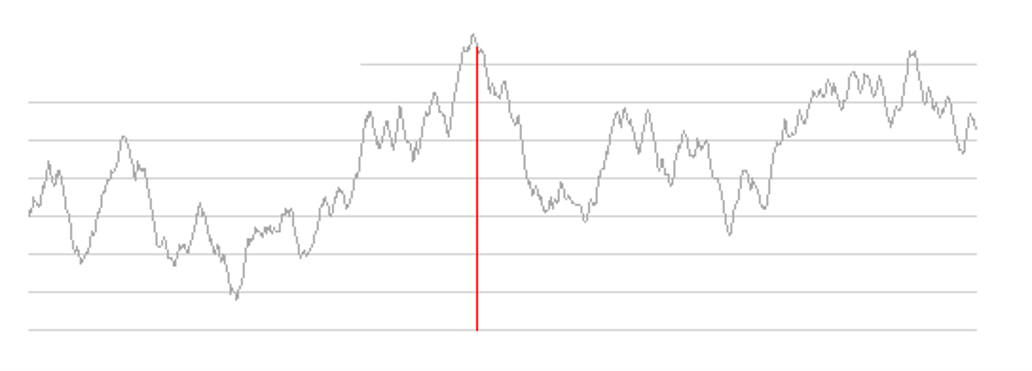
\includegraphics[width=0.9\textwidth]{pic/random.png}
    \end{figure}

    \pause
    太复杂了,完全用不了三分法。
\end{frame}

\begin{frame}{模拟退火}
    \small
    模拟退火的基本想法如下:
    \begin{itemize}
        \item 假设当前位置是 $x$,“温度”是 $T$,在 $[x-T,x+T]$ 中随机选取一个新位置 $x_\text{new}$;
        \pause
        \item 如果新位置更小,就把 $x$ 更新为 $x_\text{new}$;否则 \textbf{“抛硬币”} 来决定是否把 $x$ 更新为 $x_\text{new}$;
        \pause
        \item 逐步缩小 $T$,最后收敛到某个位置。
    \end{itemize}
    \pause
    “抛硬币”是为了防止程序在陷入局部最优点之后不愿意出来寻找更优点。\pause 这个硬币是一枚特殊的硬币,
    它有 $p$ 的概率出现正面,$1-p$ 的概率出现反面,其中
    \begin{equation*}
        p=e^{-\frac{f(x_\text{new})-f(x)}{T}},
    \end{equation*}
    抛到正面就更新,反面就不更新。
\end{frame}

\begin{frame}[fragile]{模拟退火代码}
    \small
    \begin{lstlisting}[language=c++]
        double f(double x){return ...}
        double RAND(){return (double)rand() / RAND_MAX;}
        double accept(double dta,double tem){
            return dta < 0 || RAND() < exp(-dta/tem);
        }
        // tem: 初温; delta: 降温系数; end: 终温;
        void anneal(double pnt, double tem, double delta, double end)
        {
            double ans = f(pnt);
            while(tem > end)
            {
                double nxt = pnt + tem * (RAND()*2-1);
                double nxtans = f(nxt);
                if(accept(nxtans-ans, tem)) pnt = nxt;
                tem *= delta;
            }
        }
    \end{lstlisting}

    \begin{equation*}
        \text{循环次数}=\log_{\text{降温系数}}\frac{\text{终温}}{\text{初温}}.
    \end{equation*}
\end{frame}

\begin{frame}{模拟退火的调参}
    \small
    模拟退火的三个参数一般按如下方式选择:
    \begin{itemize}
        \item 初温是可行解空间的尺寸;
        \item 终温是精度要求的 $0.1$ 倍;
        \item 降温系数要保证程序运行时间足够久,但又不能超时。
    \end{itemize}
\end{frame}

\begin{frame}{模拟退火的技术}
    \small
    模拟退火有以下优化技巧:
    \begin{itemize}
        \item \textbf{记录最优解}:用一个全局变量保存每一次计算中的最小值;
        \item \textbf{卡时}:重复退火,直到即将TLE为止;
        \item \textbf{局部迭代}:在退火结束后把温度固定为终温,重复循环若干次。
    \end{itemize}
\end{frame}

\begin{frame}[fragile]{实用的模拟退火板子}
    \footnotesize
    \begin{lstlisting}[language=c++]
        double f(double x){
            double res = ...;
            if(res < ans) ans = res, ansx = x; // 记录最优解
            return res;
        }
        double RAND(){return (double)rand() / RAND_MAX;}
        double accept(double dta,double tem){
            return dta < 0 || RAND() < exp(-dta/tem);
        }
        // tem: 初温; delta: 降温系数; end: 终温;
        void anneal(double pnt, double tem, double delta, double end){
            double local_ans = f(pnt);
            while(tem > end){
                double nxt = pnt + tem * (RAND() * 2 - 1);
                double nxtans = f(nxt);
                if(accept(nxtans-local_ans, tem)) pnt = nxt;
                tem *= delta;
            }
            for(int i = 1; i <= 1000; i++)  // 局部迭代1000次
                f(ansx + tem * (RAND() * 2 - 1));
        }
        bool TLE(){ // 卡时 0.9 秒
            return (double)(clock() - begint) / CLOCKS_PER_SEC > 0.9;
        }
    \end{lstlisting}
\end{frame}

\begin{frame}{P1337 [JSOI2004] 平衡点}
    \small
    \begin{figure}[H]
        \centering
        \begin{minipage}[t]{0.49\textwidth}
            \centering
            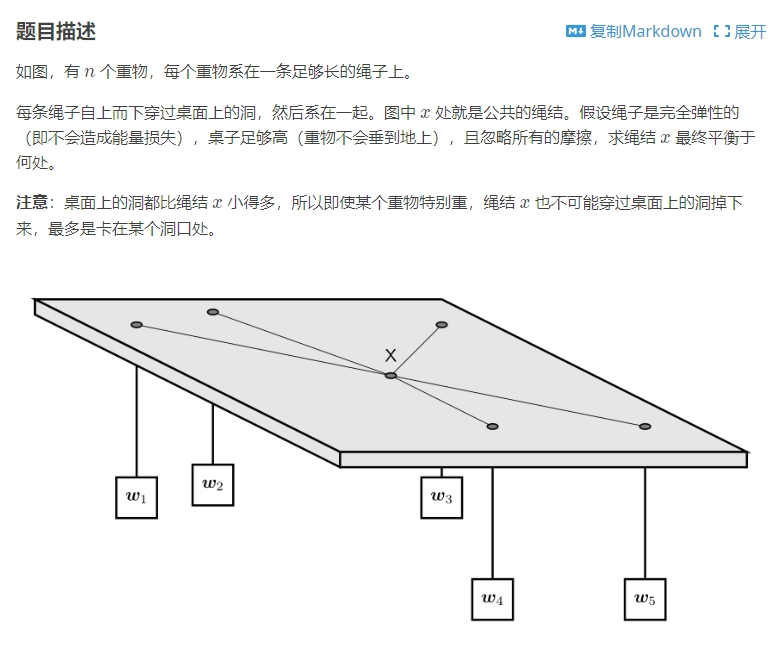
\includegraphics[width=\textwidth]{pic/p1337_1.png}
        \end{minipage}
        \hfill
        \begin{minipage}[t]{0.49\textwidth}
            \centering
            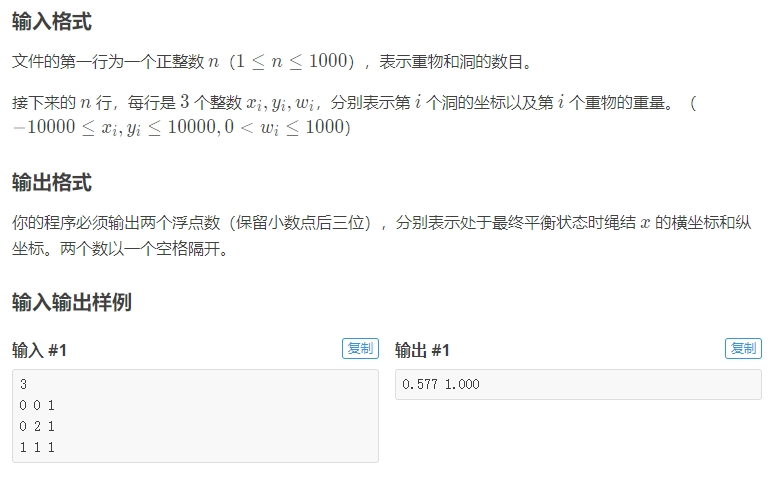
\includegraphics[width=\textwidth]{pic/p1337_2.png}
        \end{minipage}
    \end{figure}
\end{frame}

\begin{frame}{P1337 [JSOI2004] 平衡点}
    \small
    看上去是要求“合力为零”的点,但模拟退火能做的事情是“求最小值”,如何转化?

    \pause
    实际上,我们可以求“势能最小”的点。第 $i$ 个重物提供的势能是 $w_iL_i$,其中 $L_i$ 是绳结离第 $i$ 个洞的距离。
    假设绳结的位置是 $(x,y)$,我们要求势能函数
    \begin{equation*}
        F(x,y)=\sum_{i=1}^n w_i \sqrt{(x-x_i)^2+(y-y_i)^2}
    \end{equation*}
    的最小值。

    \pause
    模拟退火即可,如果没有一次AC可以尝试调参。
\end{frame}

\begin{frame}{P5544 [JSOI2016] 炸弹攻击1}
    \small
    \begin{figure}[H]
        \centering
        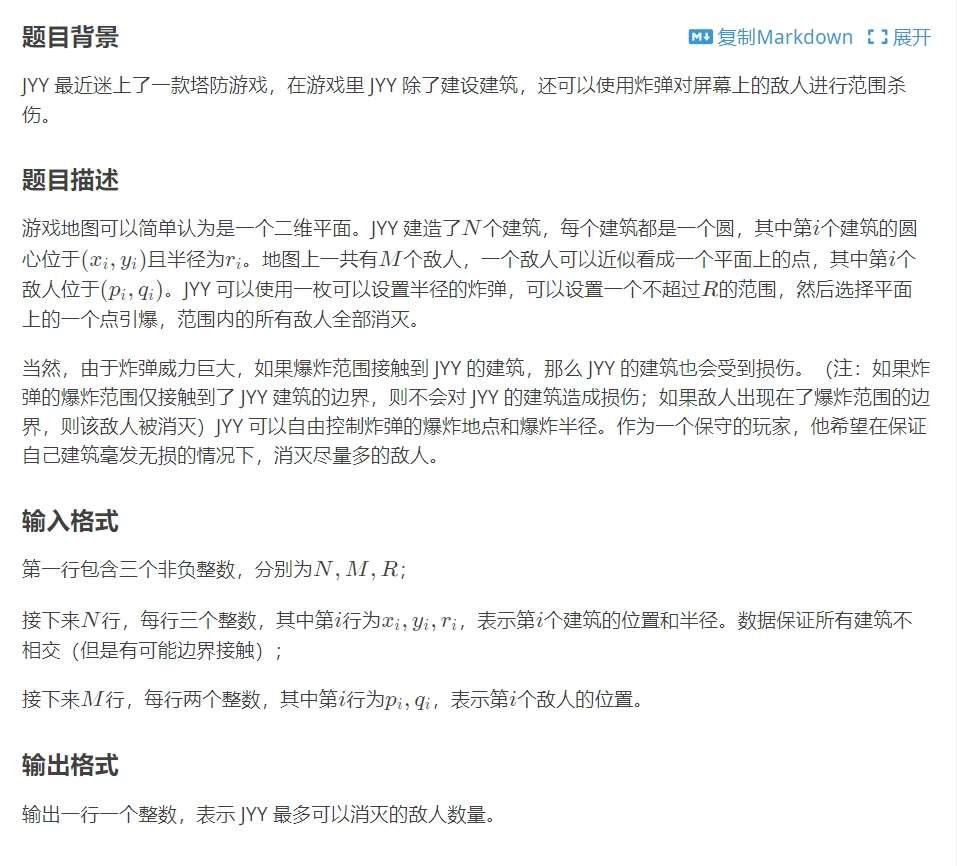
\includegraphics[width=0.8\textwidth]{pic/p5544.png}
    \end{figure}
\end{frame}

\begin{frame}{P5544 [JSOI2016] 炸弹攻击1}
    \small
    位置确定之后,把建筑遍历一遍就知道最大的可爆炸半径是多少,再枚举一遍敌人即可算出被消灭的人数。
    \vspace{1em}
    \pause
    用模拟退火来确定位置即可。
\end{frame}

\begin{frame}{开始!}
    \small
    到此为止,我们介绍的都是模拟退火的正确用法,这里的“正确”是指:
    从概率论的角度可以证明这么做的正确性。

    \pause
    接下来,我们将介绍模拟退火的一些“错误”用法,它可以帮助你在毫无思路
    的时候“骗取”更多的分数。
\end{frame}

\begin{frame}{旅行商问题}
    \small
    在一个带边权的完全无向图中,找一个权值和最小的哈密顿回路。
    \vspace{1em}
    “哈密顿回路”是指经过每个点恰好一次的环。
    \vspace{1em}
    这是经典的 NPC 问题,目前为止没有多项式复杂度的正确算法。
\end{frame}

\begin{frame}[fragile]{旅行商问题}
    \small
    可以使用模拟退火。先随机产生一个排列,然后每次迭代随机交换两个点的位置,
    再根据退火的准则来决定是否接受新的解。

    \vspace{1em}
    \begin{lstlisting}[language=c++]
    void anneal(vector<int> pnt, double tem, double delta, double end){
        double local_ans = f(pnt);
        vector<int> nxt;
        while(tem > end){
            nxt = pnt;
            swap(nxt[rand()%n], nxt[rand()%n]);
            double nxtans = f(nxt);
            if(accept(nxtans-local_ans, tem)) pnt = nxt;
            tem *= delta;
        }
    }
    \end{lstlisting}

\end{frame}

\begin{frame}{最大团问题}
    \small
    求无向图的最大团。
    \vspace{1em}
    “团”是指:在图里选出若干个点,这些点两两之间都有连边。
    “最大团”就是最大的团。
\end{frame}

\begin{frame}{最大团问题}
    \small
    还是模拟退火。每次迭代往当前团中随机添加一个新的点,
    然后将原团中与新点不相连的点移出,得到一个新团。
    将新团的大小与原团的大小比较,根据退火准则决定是否接受新解。
\end{frame}

\begin{frame}{P3959 [NOIP2017] 宝藏}
    \small
    \begin{figure}[H]
        \centering
        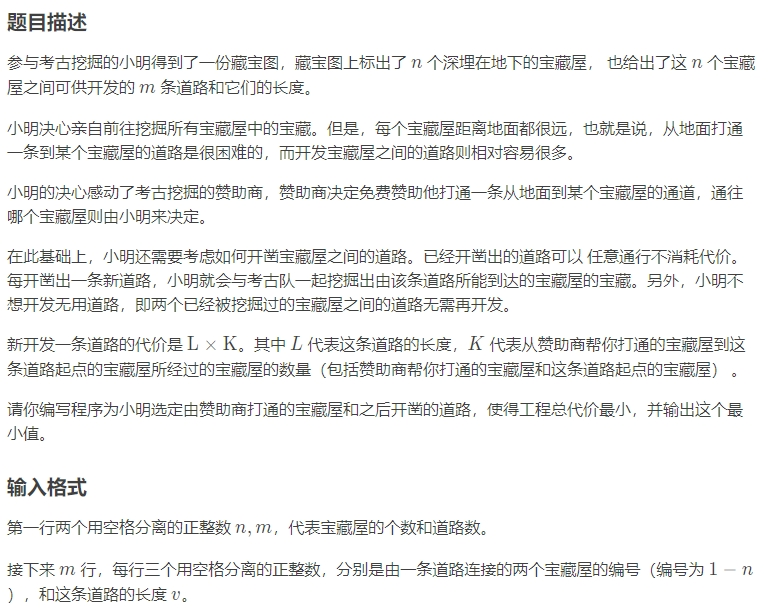
\includegraphics[width=0.8\textwidth]{pic/p3959.png}
    \end{figure}
\end{frame}

\begin{frame}[fragile]{P3959 [NOIP2017] 宝藏}
    \small
    如果已经知道了宝藏屋之间的树形结构,计算总代价显然是很简单的。
    我们考虑用模拟退火来确定这个树形结构。

    \vspace{1em}\pause
    \begin{lstlisting}[language=c++]
    void anneal(int root,double tem,double delta,double end){
        int res=calc(root);
        while(tem>end){
            int x=rand()%n+1,y=rand()%n+1;
            while(x==y||x==root) x=rand()%n+1,y=rand()%n+1;
            int pre=fa[x];fa[x]=y;  // 随机更换某个节点的父亲
            if(!check()){fa[x]=pre;continue;}  // 若更换后不再是树形结构,重新随机
            LL nxt=calc(root);
            if(accept(nxt-res,tem)) res=nxt;  // 用退火准则来决定是否接受新解
            else fa[x]=pre;
            tem*=delta;
        }
    }
    \end{lstlisting}

\end{frame}

\begin{frame}{P3878 [TJOI2010] 分金币}
    \small
    \begin{figure}[H]
        \centering
        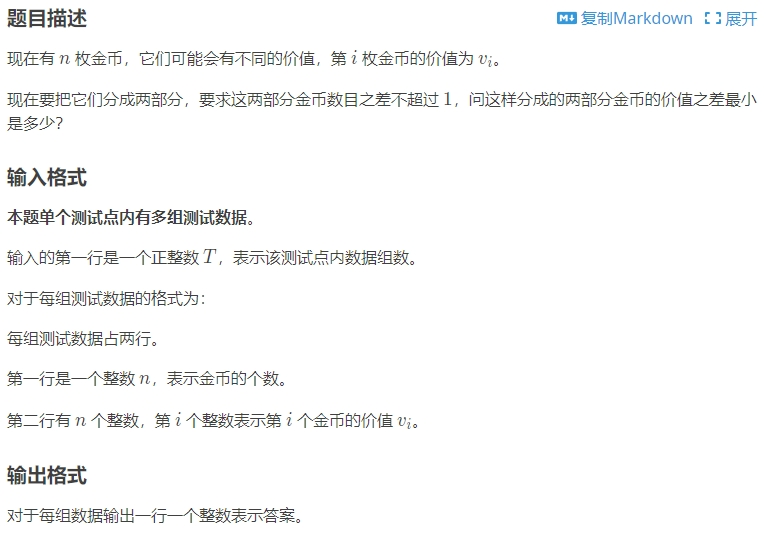
\includegraphics[width=0.8\textwidth]{pic/p3878.png}
    \end{figure}
\end{frame}

\begin{frame}{P3878 [TJOI2010] 分金币}
    \small
    第一组金币的数量是 $n_1=\left\lfloor\frac{n}{2}\right\rfloor$,
    第二组金币的数量是 $n_2=n-n_1$。

    \vspace{1em}\pause
    模拟退火,每次迭代随机交换第一组中的某个金币和第二组中的某个金币,
    然后把新的价值差和原来的价值差比较,根据退火准则决定是否接受新解。
\end{frame}


\begin{frame}
    \begin{center}
        {\Huge\calligra Thank You}
    \end{center}
\end{frame}

\end{document}